\begin{figure}[htbp]
\centering
\begin{tikzpicture}[x=1cm,y=1cm]
\node[anchor=south west,inner sep=0] at (0,0) {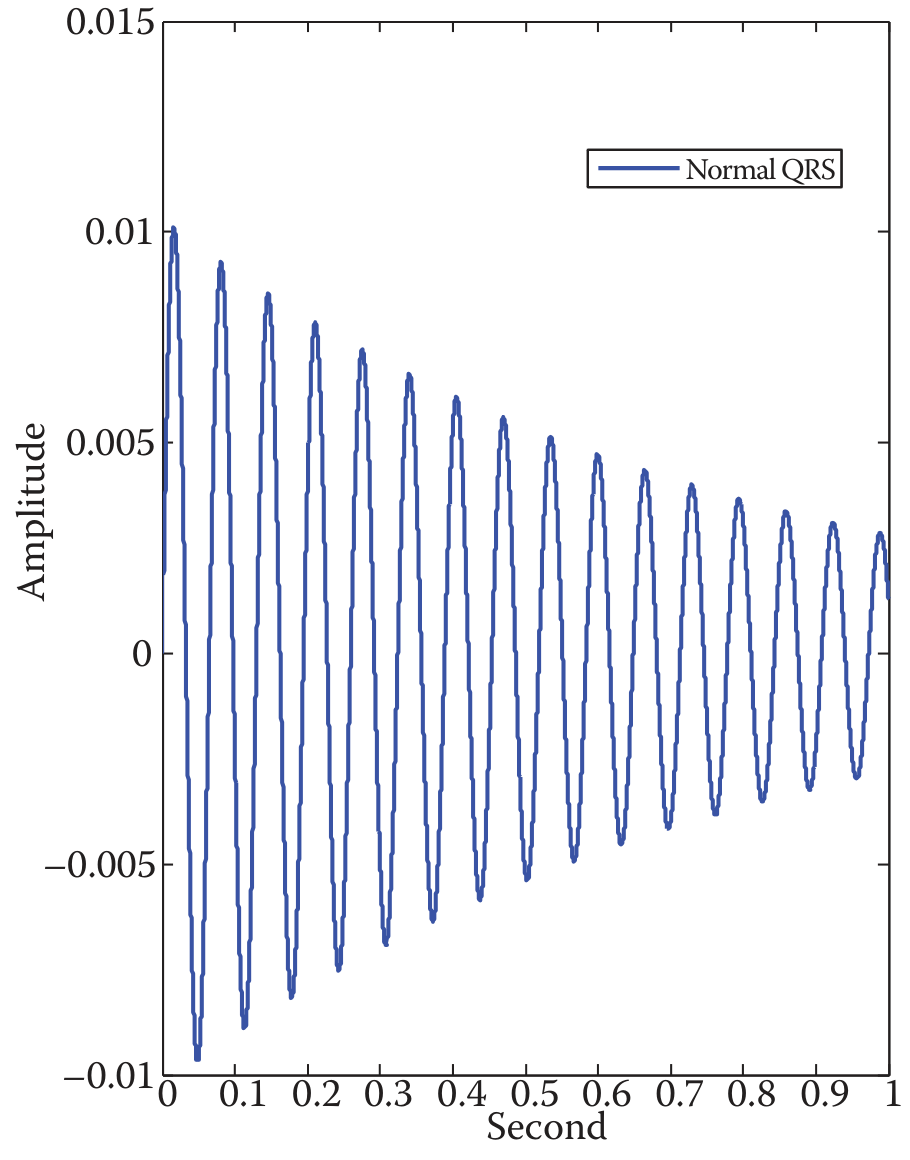
\includegraphics[width=9.0cm]{figures/ch03_fig06_data.png}};
\fill[white] (6.7747,9.6527) rectangle (8.2879,9.9692);
\fill[white] (4.7771,0.0876) rectangle (6.0391,0.5327);
\node[font=\scriptsize,rotate=0,inner sep=0] at (5.4081,0.3102) {时间（秒）};
\fill[white] (0.1122,5.4948) rectangle (0.5672,7.3185);
\node[font=\scriptsize,rotate=90,inner sep=0] at (0.3397,6.4066) {振幅};
\node[font=\scriptsize,rotate=0,inner sep=0] at (7.5230,9.7811) {正常 QRS};
\end{tikzpicture}
\origfig{6}{异常 QRS 波群所对应心脏系统的单位阶跃响应曲线。}
\label{fig:ch03-06}
\end{figure}
